\chapter{Đại số boolean}

Boolean (hay luận lý) chỉ giá trị đúng hoặc sai của mệnh đề nào đó. 
Theo cách hiểu cơ bản, boolean gồm hai giá trị 0 hoặc 1 (sai hoặc đúng). Chương này tham khảo chính từ \cite{Tokareva1} và \cite{Tokareva2}.

\section{Hàm boolean}

Hàm boolean $f$ đối với các biến $x_1, x_2, \ldots, x_n$ là hàm số 
nhận giá trị trong $\FF_2^n$ và trả về giá trị thuộc $\FF_2$.

Nói cách khác $f$ là ánh xạ từ $\FF_2^n$ tới $\FF$.

Ta ký hiệu hàm boolean $n$ biến là $f(x_1, x_2, \ldots, x_n)$.

Do $x_i \in \FF_2$ nên ta có $2^n$ vector (bộ số)
$(x_1, x_2, \ldots, x_n)$. Giá trị của hàm $f$ lại nằm
trong tập $\{0, 1\}$ nên ứng với mỗi vector có thể có 2 giá 
trị của hàm boolean, và ta có $2^n$ vector nên số lượng hàm
boolean có thể có là $2^{2^n}$.

Một số toán tử boolean hay dùng: đối, AND, OR, XOR, NAND, NOR, 
kéo theo, tương đương.

Để biểu diễn hàm boolean chúng ta dùng bảng chân trị. Bảng chân
trị tương ứng với các toán tử boolean trên là:

\begin{table}[ht]
    \centering
    \begin{tabular}{|c|c|c|c|c|c|c|}
        \hline
        & & AND & OR & XOR & NAND & NOR \\
        $x_1$ & $x_2$ & $x_1 \cdot x_2$ & $x_1 \vee x_2$ &
            $x_1 \oplus x_2$ & $x_1 \vert x_2$ &
            $x_1 \downarrow x_2$ \\
        \hline
        0 & 0 & 0 & 0 & 0 & 1 & 1 \\
        \hline
        0 & 1 & 0 & 1 & 1 & 1 & 0 \\
        \hline
        1 & 0 & 0 & 1 & 1 & 1 & 0 \\
        \hline
        1 & 1 & 1 & 1 & 0 & 0 & 0 \\
        \hline
    \end{tabular}
    \caption{Các toán tử AND, OR, XOR, NAND, NOR}
\end{table}

Toán tử đối làm đổi giá trị của hàm bool (0 thành 1 và 1 thành 0).
Ký hiệu $\overline{x}$.

\begin{table}[ht]
    \begin{subtable}[t]{0.25\textwidth}
        \centering
        \begin{tabular}{|c|c|}
            \hline
            $x$ & $\overline{x}$ \\
            \hline
            0 & 1 \\
            \hline
            1 & 0 \\
            \hline
        \end{tabular}
        \caption{Toán tử đối}
    \end{subtable}
    \hspace{\fill}
    \begin{subtable}[t]{0.55\textwidth}
        \centering
        \begin{tabular}{|c|c|c|c|}
            \hline
            $x_1$ & $x_2$ & $x_1 \rightarrow x_2$ & $x_1 \sim x_2$ \\
            \hline
            0 & 0 & 1 & 1 \\
            \hline
            0 & 1 & 1 & 0 \\
            \hline
            1 & 0 & 0 & 0 \\
            \hline
            1 & 1 & 1 & 1 \\
            \hline
        \end{tabular}
        \caption{Toán tử kéo theo và tương đương}
    \end{subtable}
    \caption{Các toán tử đối, kéo theo, tương đương}
\end{table}

Toán tử tương đương còn chỉ sự tương đương của hai mệnh đề logic.
Khi hai biểu thức logic có cùng bảng chân trị thì hai mệnh đề đó
tương đương nhau. Do đó ta có thể viết một số kết quả như sau (từ
các bảng chân trị cơ bản trên):

\begin{itemize}
    \item $x_1 \vert x_2 \sim \overline{x_1 \cdot x_2}$. Ở đây
        ta đổi dấu từng giá trị hàm boolean $x_1 \cdot x_2$
    \item $x_1 \downarrow x_2 \sim \overline{x_1 \vee x_2}$. 
        Tương tự ta đổi dấu từng giá trị hàm boolean $x_1 \vee x_2$
\end{itemize}

\subsection*{Đa thức Zhegalkin}

\begin{definition}[Đa thức Zhegalkin]
    Với hàm boolean $n$ biến $f(x_1, x_2, \ldots, x_n)$, \textbf{đa thức Zhegalkin} tương ứng với hàm bool đó là cách biểu diễn
    đa thức đó dưới dạng tổng các tích như sau
    \begin{equation}
        f(x_1, x_2, \ldots, x_n) = a_0 \oplus a_1 x_1 
        \oplus a_2 x_2 \oplus a_3 x_1 x_2 \oplus \ldots 
        \oplus a_k x_1 x_2 \ldots x_n
    \end{equation}
    với $a_i \in \{0, 1\}$. Ta thấy rằng có $n$ biến, do đó có 
    $2^n$ hệ số $a_i$ ($k = 0, 1, \ldots, 2^n-1$).
\end{definition}

Khi đó ta nói hàm boolean $f$ được biểu diễn ở \textbf{dạng chuẩn tắc đại số} (algebraic normal form).

\begin{example}
    Cho hàm bool $f(x, y) = x \vee y$. Ta có bảng chân trị sau
    \begin{table}[ht]
        \centering
        \begin{tabular}{|c|c|c|}
            \hline
            $x$ & $y$ & $f(x, y)$ \\ \hline
            0 & 0 & 0 \\ \hline
            0 & 1 & 1 \\ \hline
            1 & 0 & 1 \\ \hline
            1 & 1 & 1 \\ \hline
        \end{tabular}
    \end{table}

    Bảng chân trị này tương đương với đa thức Zhegalkin
    \[f(x, y) = x \oplus y \oplus xy\]
\end{example}

\begin{definition}[Bậc của đa thức Zhegalkin]
    Tương tự như bậc của một đa thức đại số thông thường,
    bậc của đa thức Zhegalkin là bậc của hạng tử chứa nhiều
    đơn thức $x_i$ nhất. Ký hiệu là $\deg(f)$.
\end{definition}

\begin{example}
    Xét hàm boolean $f(x, y, z) = 1 \oplus x \oplus yz \oplus xyz$.
    Khi đó $\deg(f) = 3$ vì hạng tử chứa nhiều đơn thức nhất là $xyz$
    có 3 đơn thức.

    Xét hàm boolean $f(x, y, z) = 1 \oplus z \oplus zy \oplus xy$. 
    Khi đó $\deg(f) = 2$ vì hạng tử chứa nhiều đơn thức nhất là
    $zy$ (cũng có thể xét $xy$).
\end{example}

\subsection*{Cách tìm đa thức Zhegalkin từ bảng chân trị}

Ta có nhiều phương pháp để tìm đa thức Zhegalkin của một hàm 
boolean từ bảng chân trị. 

\subsubsection*{Phương pháp tam giác}

Ở hàng đầu ta viết các phần
tử bảng chân trị từ trái sang phải. Với $n$ biến sẽ có $2^n$ ô.
Hàng thứ hai có $2^n-1$ ô. Phần tử dưới sẽ bằng XOR của 2 phần tử 
ngay trên nó (tạo thành tam giác). Tiếp tục như vậy tới khi
ta có hàng cuối chỉ có 1 ô.

\begin{figure}[ht]
    \centering
    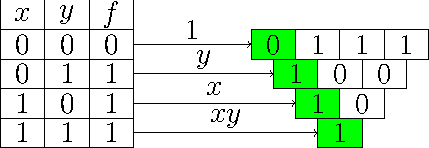
\includegraphics[page=1]{figures/boolean/zhegalkin.pdf}
    \caption{Phương pháp tam giác}
\end{figure}

Khi đó, tương ứng với các biến, nếu biến đó là 1 thì hạng tử chứa
biến đó, 0 thì không ghi. Ở ví dụ trên, nếu $(x, y) = (0, 0)$ 
thì không có gì (phần tử 1), $(x, y) = (0, 1)$ tương ứng với hạng 
tử $y$ trong đa thức Zhegalkin, $(x, y) = (1, 0)$ tương ứng hạng
tử $x$. Cuối cùng $(x, y) = (1, 1)$ tương ứng hạng tử $xy$.

Hệ số trước mỗi hạng tử là phần tử đầu tiên bên trái theo bảng
kim tự tháp. Như vậy đa thức Zhegalkin là:
\begin{equation*}
    f(x, y) = 0 \cdot 1 \oplus 1 \cdot y \oplus 1 \cdot x \oplus 
        1 \cdot xy = x \oplus y \oplus xy
\end{equation*}

Đa thức Zhegalkin đóng vai trò quan trọng trong nhiều lĩnh vực,
bao gồm cả toán học, vật lý, khoa học máy tính, vì AND và XOR
là hai toán tử đại số cơ bản, do đó biểu diễn đa thức Zhegalkin
được gọi là dạng chuẩn tắc đại số như ở trên đề cập.

Một ví dụ khác của đa thức Zhegalkin với hàm 3 biến $x$, $y$ và $z$
như hình sau:

\begin{figure}[ht]
    \centering
    \includegraphics[page=2]{figures/boolean/zhegalkin.pdf}
\end{figure}

Như vậy ứng với hàm boolean $f$ thì đa thức Zhegalkin là:
\begin{equation*}
    f(x, y, z) = z \oplus yz \oplus x \oplus xz \oplus xyz
\end{equation*}

\subsubsection*{Phương pháp Möbius}

Phương pháp này cho phép chúng ta tính hệ số đa thức Zhegalkin
như phương pháp tam giác nhưng nhanh hơn và đỡ sai sót hơn.

Đầu tiên chúng ta chia đôi bảng chân trị thành hai nửa trái phải.
Nửa trái giữa nguyên, mỗi phần tử ở nửa phải được XOR (cộng modulo 2)
với phần tử tương ứng ở nửa trái.

Giả sử với hàm $f(x, y) = (0, 1, 1, 1)$ như trên. Bước 1, ta giữ
nguyên 2 phần tử đầu 0 và 1. Phần tử thứ ba (mới) bằng
phần tử thứ ba (cũ) XOR với phần tử đầu ($0 \oplus 1 = 1$).
Phần tử thứ tư (mới) bằng phần tử thứ tư (cũ) XOR với phần tử
thứ hai ($1 \oplus 1 = 0$).

Tiếp theo, chúng ta xử lý như trên cho 2 phần tử bên nửa trái 
(2 phần tử bên nửa phải xử lý tương tự).

\begin{figure}[ht]
    \begin{subfigure}{0.45\textwidth}
        \centering
        \includegraphics[page=3]{figures/boolean/zhegalkin.pdf}
        \caption{Bước 1}
    \end{subfigure}
    \hfill
    \begin{subfigure}{0.45\textwidth}
        \centering
        \includegraphics[page=4]{figures/boolean/zhegalkin.pdf}
        \caption{Bước 2}
    \end{subfigure}
\end{figure}

Như vậy ta có kết quả là $(0, 1, 1, 1)$, tương ứng với các
hạng tử $1$, $y$, $x$, $xy$ (như trên). Vậy đa thức Zhegalkin
là $f(x, y) = x \oplus y \oplus xy$.

\subsection*{Hàm affine và hàm tuyến tính}

\begin{definition}[Hàm boolean affine]
    Xét hàm boolean $n$ biến $f(x_1, x_2, \ldots, x_n)$.
    Khi đó $f$ được gọi là \textbf{hàm boolean affine} nếu nó có dạng
    \begin{equation}
        f(x_1, x_2, \ldots, x_n) = a_0 \oplus a_1 x_1 \oplus 
        a_2 x_2 \oplus \ldots \oplus a_n x_n
    \end{equation}
    Khi $a_0 = 0$ thì ta gọi là \textbf{hàm boolean tuyến tính}
    (linear).
\end{definition}

Ta thấy rằng chỉ có các hạng tử dạng $a_i x_i$ xuất hiện trong
biểu diễn đa thức Zhegalkin tương ứng của hàm boolean đó. Hay 
nói cách khác hàm boolean là affine khi $\deg(f) = 1$.

\begin{example}
    Hàm boolean $f(x, y) = x \oplus y$ là hàm boolean affine và cũng tuyến tính. Hàm boolean $f(x, y) = x \oplus xy$ không là hàm boolean affine.
\end{example}

Tiếp theo ta sẽ xét sự so sánh của hai vector và hàm boolean đơn điệu.

\subsection*{Hàm đơn điệu}

\begin{definition}[Vector so sánh được]
    Xét hai vector $\bm{a} = (a_1, a_2, \ldots, a_n)$ và $\bm{b} = (b_1, b_2, \ldots, b_n)$ ($a_i, b_i \in \{0, 1\}$). 
    Ta nói $\bm{a}$ \textbf{so sánh được nhỏ hơn} $\bm{b}$ nếu với mọi $i = 1, 2, \ldots, n$
    ta có $a_i \leqslant b_i$. Ký hiệu $\bm{a} \prec \bm{b}$.
\end{definition}

\begin{example}
    Ta có $(1, 0, 0) \prec (1, 0, 1)$, còn $(1, 0, 0)$ và $(0, 1, 0)$
    thì không so sánh được (vị trí thứ 1 và thứ 2).
\end{example}

\begin{definition}[Hàm boolean đơn điệu]
    Hàm boolean $n$ biến $f(x_1, x_2, \ldots, x_n)$ được gọi là \textbf{hàm boolean đơn điệu} (monotone) nếu với mọi vector $(a_1, a_2, \ldots, a_n) \prec (b_1, b_2, \ldots, b_n)$ thì ta có 
    \begin{equation}
        f(a_1, a_2, \ldots, a_n) \leqslant f(b_1, b_2, \ldots, b_n)  
    \end{equation}
\end{definition}

\begin{example}
    Xét hàm boolean $f(x, y) = (0, 1, 0, 1)$.

    Ta thấy rằng:
    \begin{itemize}
        \item $(0, 0) \prec (0, 1)$ và $f(0, 0) = 0 \leqslant 1 = f(0, 1)$
        \item $(0, 0) \prec (1, 0)$ và $f(0, 0) = 0 \leqslant 0 = f(1, 0)$
        \item $(0, 0) \prec (1, 1)$ và $f(0, 0) = 0 \leqslant 1 = f(1, 1)$
        \item $(0, 1)$ và $(1, 0)$ không so sánh được nên bỏ qua
        \item $(0, 1) \prec (1, 1)$ và $f(0, 1) = 1 \leqslant 1 = f(1, 1)$
        \item $(1, 0) \prec (1, 1)$ và $f(1, 0) = 0 \leqslant 1 = f(1, 1)$
    \end{itemize}

    Vậy đây là hàm đơn điệu.
\end{example}

\section{Trọng số, phổ Furier, phổ Walsh, Hamming distance}

Ở phần này ký hiệu vector không $\bm{0} = (0, \ldots, 0)$, vector một $\bm{1} = (1, \ldots, 1)$.

\subsection*{Trọng số của hàm boolean}

\begin{definition}[Trọng số hàm boolean]
	\textbf{Trọng số} (hay \textbf{weight}) của hàm boolean $n$ biến $f(x_1, x_2, \ldots, x_n)$ là số lượng giá trị khác 0 của hàm $f$. 
    
    Ký hiệu là $\wt(f)$.
\end{definition}

\begin{example}
	Hàm boolean $f(x, y) = (0, 1, 0, 1)$ có trọng số $\wt(f) = 2$.
	Hàm boolean $f(x, y, z) = (1, 0, 1, 1, 1, 0, 0, 1)$ có trọng số $\wt(f) = 5$.
\end{example}

Một số tính chất của trọng số:

\begin{enumerate}
	\item $0 \leqslant \wt(f) \leqslant 2^n$
	\item $\wt(f \oplus \bm{1}) = 2^n - \wt(f)$
	\item Nếu $h$ cũng là một hàm boolean từ $\FF_2^n$ tới $\FF_2$ thì \[\wt(f \oplus h) = \wt(f) + \wt(h) - 2 \wt(fh)\]
	\item Giá trị $\wt(f)$ nhận giá trị lẻ khi và chỉ khi $\deg(f) = n$
\end{enumerate}

\subsection*{Biến đổi Fourier}

Với mỗi vector $\bm{a} = (a_1, \ldots, a_n) \in \FF_2^n$, ta ký
hiệu $\langle \bm{a}, \bm{x} \rangle$ là hàm sau:
\begin{equation}\label{fur:eq1}
	\langle \bm{a}, \bm{x} \rangle = a_1 x_1 \oplus a_2 x_2 \oplus \ldots \oplus a_n x_n
\end{equation}

Mỗi hàm boolean $f(\bm{x}) = f(x_1, x_2, \ldots, x_n)$ sẽ được biểu diễn dưới dạng duy nhất với
\begin{equation}\label{fur:eq2}
	f(\bm{x}) = 2^{-n} \sum_{\bm{a} \in \FF_2^n} F_f (\bm{a}) \cdot (-1)^{\langle \bm{a}, \bm{x} \rangle}
\end{equation}

Trong đó
\begin{equation}\label{fur:eq3}
	F_f (\bm{a}) = \sum_{\bm{x} \in \FF_2^n} f(\bm{x}) \cdot (-1)^{\langle \bm{a}, \bm{x} \rangle}
\end{equation}

Khi đó, tập hợp $\{F_f (\bm{a}), \bm{a} \in \FF_2^n \}$ được gọi là 
\textbf{phổ Fourier} (spectre Fourier) của hàm boolean $f$.

\begin{remark}
	Đầu tiên ta có nhận xét rằng, với vector $\bm{z}$ cố định thì
	\begin{equation}\label{fur:eq4}
		\sum_{\bm{a} \in \FF_2^n} (-1)^{\langle \bm{a}, \bm{z} \rangle} = \begin{cases}
			0, \quad & \text{nếu } \bm{z} \neq \bm{0} \\
			2^n, \quad & \text{nếu } \bm{z} = \bm{0}
		\end{cases}
	\end{equation} 
\end{remark}

\begin{proof}
	Để chứng minh nhận xét này, ta thấy rằng nếu $\bm{z} \neq \bm{0}$ thì có ít nhất một bit $z_i \neq 0$. 
    
    Ta chọn vector $\Delta = (0, \ldots, 0, 1, 0, \ldots, 0)$ với bit 1 nằm ở vị trí $i$. Khi đó với mọi vector $\bm{a} \in \FF_2^n$ tồn tại duy nhất vector $\bm{a}' \in \FF_2^n$ sao cho $\bm{a} \oplus \bm{a}' = \Delta$. 
    
    Suy ra $\langle \bm{a} \oplus \bm{a}', \bm{z} \rangle = \langle \Delta, \bm{z} \rangle = 1$ vì $z_i \cdot 1 = 1$, các vị trí còn lại $z_j \cdot 0 = 0$. 
    
    Lý do ta chọn vector $\Delta$ như vậy là vì $\langle \bm{a} \oplus \bm{a}', \bm{z} \rangle = \langle \bm{a}, \bm{z} \rangle \oplus \langle \bm{a}', \bm{z} \rangle = 1$. Tương đương với $\langle \bm{a}, \bm{z} \rangle = 1 \oplus \langle \bm{a}', \bm{z} \rangle$. Do đó $\langle \bm{a}, \bm{z} \rangle$ và $\langle \bm{a}', \bm{z} \rangle$ là hai bit khác nhau, dẫn tới $(-1)^{\langle \bm{a}, \bm{z} \rangle}$ và $(-1)^{\langle \bm{a}', \bm{z} \rangle}$ là hai số trái dấu nhau nên tổng chúng là 0. Chúng ta có $2^n / 2$ cặp như vậy và tổng cuối cùng là 0.
	
	Trong trường hợp $\bm{z} = \bm{0}$ thì $\langle \bm{a}, \bm{z} \rangle = \bm{0}$ với mọi $\bm{a} \in \FF_2^n$. Do đó $(-1)^{\langle \bm{a}, \bm{z} \rangle} = (-1)^0 = 1$ với mọi vector $\bm{a}$. Hàm boolean $n$ biến có $2^n$ vector $\bm{a}$ nên tổng là $2^n \cdot 1 = 2^n$.
\end{proof}

Nhận xét \ref{fur:eq4} đã được chứng minh. Ta quay lại bài toán.

\begin{proof}
	Với mọi vector $\bm{x} \in \FF_2^n$, ta khai triển từ vế phải của \ref{fur:eq2} và từ \ref{fur:eq3}
	
	\begin{align*}
		& 2^{-n} \sum_{\bm{a} \in \FF_2^n} F_f (\bm{a}) \cdot (-1)^{\langle \bm{a}, \bm{x} \rangle} \\ = & 2^{-n} \sum_{\bm{a} \in \FF_2^n} \biggl( \sum_{\bm{y} \in \FF_2^n} f(\bm{y}) \cdot (-1)^{\langle \bm{a}, \bm{y} \rangle} \biggr) \cdot (-1)^{\langle \bm{a}, \bm{x} \rangle} \\ = & 2^{-n} \sum_{\bm{y} \in \FF_2^n} f(\bm{y}) \sum_{\bm{a} \in \FF_2^n} (-1)^{\langle \bm{a}, \bm{y} \oplus \bm{x} \rangle}
	\end{align*}
	
	Theo \ref{fur:eq4}, nếu ta coi $\bm{y} \oplus \bm{x} = \bm{z}$ thì 
	\begin{equation*}
		\sum_{\bm{a} \in \FF_2^n} (-1)^{\langle \bm{a}, \bm{y} \oplus \bm{x} \rangle} = \begin{cases}
			0, \quad & \text{nếu } \bm{y} \oplus \bm{x} \neq \bm{0} \\
			2^n, \quad & \text{nếu } \bm{y} \oplus \bm{x} = \bm{0}
		\end{cases}
	\end{equation*}
	
	Nghĩa là trong tổng trên thì chỉ có $\bm{y}$ thỏa $\bm{y} \oplus \bm{x} = \bm{0}$ thì $f(\bm{y})$ không bị triệt tiêu. Nói cách khác là $\bm{y} = \bm{x}$ và do đó tổng trên còn lại $2^{-n} (f(\bm{x}) \cdot 2^n) = f(\bm{x})$ và ta có điều phải chứng minh.
\end{proof}

\begin{example}
	Xét hàm boolean $f(x_1, x_2) = (1, 0, 0, 1)$.
	
	Xét $\bm{a} = (0, 0)$. Ta có:
	\begin{itemize}
		\item Với $\bm{x} = (0, 0)$, $f(\bm{x}) = 1$, $\langle \bm{a}, \bm{x} \rangle = 0 \cdot 0 + 0 \cdot 0 = 0$.
		\item Với $\bm{x} = (0, 1)$, $f(\bm{x}) = 0$, $\langle \bm{a}, \bm{x} \rangle = 0 \cdot 0 + 0 \cdot 1 = 0$
		\item Với $\bm{x} = (1, 0)$, $f(\bm{x}) = 0$, $\langle \bm{a}, \bm{x} \rangle = 0 \cdot 1 + 0 \cdot 0 = 0$
		\item Với $\bm{x} = (1, 1)$, $f(\bm{x}) = 1$, $\langle \bm{a}, \bm{x} \rangle = 0 \cdot 1 + 0 \cdot 1 = 0$
	\end{itemize}
	
	Suy ra $F_f (\bm{a}) = 1 \cdot (-1)^0 + 0 \cdot (-1)^0 + 0 \cdot (-1)^0
	+ 1 \cdot (-1)^0 = 2$ khi $\bm{a} = (0, 0)$.
	
	Tương tự, ta có các giá trị $F_f (\bm{a})$ sau:
	\begin{itemize}
		\item Với $\bm{a} = (0, 1)$, $F_f (\bm{a}) = F_f (0, 1) = 0$
		\item Với $\bm{a} = (1, 0)$, $F_f (\bm{a}) = F_f (1, 0) = 0$
		\item Với $\bm{a} = (1, 1)$, $F_f (\bm{a}) = F_f (1, 1) = 2$
	\end{itemize}
	
	Bây giờ ta đã có đủ $F_f(\bm{a})$ với $\bm{a} \in \FF_2^2$ nên ta có thể kiểm chứng với mọi $\bm{x} \in \FF_2^2$ thỏa công thức \ref{fur:eq2}.
\end{example}

\subsection*{Biến đổi Walsh-Hadamard}

Với mỗi hàm boolean $f(x_1, x_2, \ldots, x_n) = f(\bm{x})$ ta định nghĩa một hàm tương ứng như sau:
\[f^*(\bm{x}) = (-1)^{f(\bm{x})}\]

Ta định nghĩa $\langle \bm{a}, \bm{x} \rangle$ như trên, khi đó hàm $f^*(\bm{x})$ sẽ có dạng
\begin{equation}\label{walsh:eq1}
	f^*(\bm{x}) = 2^{-n} \sum_{\bm{a} \in \FF_2^n} W_f (\bm{a}) (-1)^{\langle \bm{a}, \bm{x} \rangle}
\end{equation}

Trong đó
\begin{equation}\label{walsh:eq2}
	W_f (\bm{a}) = \sum_{\bm{x} \in \FF_2^n} (-1)^{f(\bm{x}) \oplus \langle \bm{a}, \bm{x} \rangle}
\end{equation}

Tập hợp $\{ W_f (\bm{a}), \bm{a} \in \FF_2^n\}$ được gọi là \textbf{phổ Walsh} (spectre Walsh) của hàm $f(\bm{x})$. Các giá trị $W_f (\bm{a})$ được gọi là hệ số Walsh.
	
\begin{proof}
	Tương tự như trên, ta khai triển vế phải của \ref{walsh:eq1} và thay \ref{walsh:eq2} vào
	\begin{align*}
		& 2^{-n} \sum_{\bm{a} \in \FF_2^n} W_f (\bm{a}) (-1)^{\langle \bm{a}, \bm{x} \rangle} \\ = & 2^{-n} \sum_{\bm{a} \in \FF_2^n} \biggl( \sum_{\bm{y} \in \FF_2^n} (-1)^{f(\bm{y}) \oplus \langle \bm{a}, \bm{y} \rangle} \biggr) (-1)^{\langle \bm{a}, \bm{x} \rangle} \\ = & 2^{-n} \sum_{\bm{y} \in \FF_2^n} (-1)^{f(\bm{y})} \sum_{\bm{a} \in \FF_2^n} (-1)^{\langle \bm{a}, \bm{y} \oplus \bm{x} \rangle}
	\end{align*}
	
	Cũng từ \ref{fur:eq4}, tương tự như trên ta có
	\begin{equation*}
		\sum_{\bm{a} \in \FF_2^n} (-1)^{\langle \bm{a}, \bm{y} \oplus \bm{x} \rangle} = \begin{cases}
			0, & \quad \text{nếu } \bm{y} \oplus \bm{x} \neq \bm{0} \\
			2^n, & \quad \text{nếu } \bm{y} \oplus \bm{x} = \bm{0}
		\end{cases}
	\end{equation*}
	
	Do đó trong các $\bm{y} \in \FF_2^n$ thì chỉ có $\bm{y} = \bm{x}$ không bị triệt tiêu nên kết quả là $2^{-n} \cdot (-1)^{f(\bm{x})} \cdot 2^n = (-1)^{f(\bm{x})} = f^* (\bm{x})$.
\end{proof}

Các hệ số Walsh liên hệ với nhau bởi công thức

\begin{equation}
	\sum_{\bm{a} \in \FF_2^n} W_f (\bm{a}) W_f (\bm{a} \oplus \bm{d}) = 
	\begin{cases}
		2^{2n}, & \bm{d} = \bm{0} \\
		0, & \bm{d} \neq \bm{0}
	\end{cases}
\end{equation}

Trường hợp $\bm{d} = \bm{0}$ được gọi là \textbf{đẳng thức Parcel}
\begin{equation}
	\sum_{\bm{a} \in \FF_2^n} (W_f (\bm{a}))^2 = 2^{2n}
\end{equation}

\subsection*{Liên hệ giữa hệ số Fourier và hệ số Walsh}

\begin{remark}
	Quan hệ giữa hệ số Fourier và hệ số Walsh là biểu thức sau
	\begin{equation}
		W_f (\bm{a}) = 2^n \Delta (\bm{a}) - 2 F_f (\bm{a})
	\end{equation}
	với $\Delta (\bm{a}) = \begin{cases}
		1, \quad \text{nếu } \bm{a} = \bm{0} \\
		0, \quad \text{nếu } \bm{a} \neq \bm{0}
	\end{cases}$
\end{remark}

\begin{proof}
	Ta có
	\begin{align*}
		W_f (\bm{a}) + 2 F_f (\bm{a}) = & \sum_{\bm{x} \in \FF_2^n} (-1)^{f(\bm{x}) \oplus \langle \bm{a}, \bm{x} \rangle} + 2 \sum_{\bm{x} \in \FF_2^n} f(\bm{x}) (-1)^{\langle \bm{a}, \bm{x} \rangle} \\ = & \sum_{\bm{x} \in \FF_2^n} (-1)^{\langle \bm{a}, \bm{x} \rangle} [(-1)^{f(\bm{x})} + 2 f(\bm{x})]
	\end{align*}
	
	Để ý rằng, nếu $f(\bm{x}) = 0$ thì $(-1)^{f(\bm{x})} + 2 f(\bm{x}) = (-1)^0 + 2 \cdot 0 = 1$, còn nếu $f(\bm{x}) = 1$ thì $(-1)^{f(\bm{x})} + 2 f(\bm{x}) = (-1)^1 + 2 \cdot 1 = 1$. Nói cách khác biểu thức trên trở thành \[ W_f (\bm{a}) + 2 F_f (\bm{a}) = \sum_{\bm{x} \in \FF_2^n} (-1)^{\langle \bm{a}, \bm{x} \rangle} \]
	
	Từ \ref{fur:eq2} ta có
	\[ \sum_{\bm{x} \in \FF_2^n} (-1)^{\langle \bm{a}, \bm{x} \rangle} = \begin{cases}
		0, \quad &\text{nếu } \bm{a} \neq \bm{0} \\ 2^n, \quad & \text{nếu } \bm{a} = \bm{0}
	\end{cases} \]
	
	Như vậy nếu đặt $\Delta(\bm{a}) = \begin{cases}
		1, \text{nếu } \bm{a} = \bm{0} \\ 0, \text{nếu } \bm{a} \neq \bm{0}
	\end{cases}$ thì ta có điều phải chứng minh.
\end{proof}
	
\begin{remark}
	Khi $\bm{a} = \bm{0}$ thì với mọi $\bm{x} \in \FF_2^n$ ta đều có $\langle \bm{a}, \bm{x} \rangle = 0$. Do đó \[F_f (\bm{0}) = \sum_{\bm{x} \in \FF_2^n} f(\bm{x}) (-1)^{\langle \bm{a}, \bm{x} \rangle} = \sum_{\bm{x} \in \FF_2^n} f(\bm{x}) (-1)^0 = wt(f)\]
	
	Suy ra 
	\begin{equation}\label{walsh:eq4}
		W_f (\bm{0}) = 2^n - 2 wt(f) \Leftrightarrow wt(f) = 2^{n-1} - \frac{1}{2} W_f (\bm{0})
	\end{equation}
\end{remark}
	
\subsection*{Khoảng cách Hamming}

\begin{definition}[Khoảng cách Hamming giữa hai vector]
	Với hai vector $\bm{x}$, $\bm{y}$ thuộc $\FF_2^n$, đặt
	\begin{equation}
		d (\bm{x}, \bm{y}) = \wt (\bm{x} \oplus \bm{y})
	\end{equation}
	là \textbf{khoảng cách Hamming} giữa hai vector $\bm{x}$ và $\bm{y}$. Trong đó $\wt(\bm{z})$ là trọng số vector $\bm{z}$.
\end{definition}

\begin{definition}[K/cách Hamming từ vector tới tập vector]
	Xét $M \subseteq \FF_2^n$. Khi đó với mọi $\bm{x} \in \FF_2^n$, ta nói khoảng cách từ $\bm{x}$ tới $M$ là
	\begin{equation}
		d(\bm{x}, M) = \min_{\bm{y} \in M} d (\bm{x}, \bm{y})
	\end{equation}
\end{definition}

\begin{definition}[Khoảng cách Hamming giữa hai hàm boolean]
	Xét hai hàm boolean $n$ biến là $f(x_1, x_2, \ldots, x_n)$ và $g(x_1, x_2, \ldots, x_n)$. Khi đó khoảng cách Hamming từ hàm $f$ tới hàm $g$ là
	\begin{equation}
		d(f, g) = \wt(f \oplus g) = \sum_{\bm{x} \in \FF_2^n} f(\bm{x}) \oplus g(\bm{x})
	\end{equation}
\end{definition}

\subsection*{Hàm Bent}

Ta ký hiệu $\mathcal{L}$ là tập hợp tất cả các hàm boolean affine với $n$ biến. Nghĩa là

\begin{equation}
	\mathcal{L} = \{ l_{a_0} (\bm{a}, \bm{x}) \, | \, a_0 \in \FF_2, \bm{a} \in \FF_2^n \}
\end{equation}
với $l_{a_0} (\bm{a}, \bm{x}) = a_0 \oplus a_1 x_1 \oplus \ldots \oplus a_n x_n$.

\begin{definition}[Nonlinearity của hàm boolean]
	\textbf{Nonlinearity} của hàm boolean $f$ bất kì được định nghĩa là khoảng cách Hamming từ $f$ tới $\mathcal{L}$, hay nói cách khác $N_f = d(f, \mathcal{L})$.
\end{definition}

\begin{remark}
	Xét hàm $f$ với $n$ biến và phổ Walsh tương ứng của hàm $f$ là $\{ W_f (\bm{a}), \bm{a} \in \FF_2^n \}$. Khi đó 
	
	\begin{equation}\label{walsh:eq3}
		N_f = 2^{n-1} - \frac{1}{2} \max_{\bm{a} \in \FF_2^n} \lvert W_f (\bm{a}) \rvert
	\end{equation}
\end{remark}

\begin{remark}
	Từ đẳng thức Parcel ta có 
	\begin{align*}
		& 2^n \cdot \bigl(\max_{\bm{a} \in \FF_2^n} (W_f (\bm{a}))^2\bigr) \geqslant \sum_{\bm{a} \in \FF_2^n} (W_f (\bm{a}))^2 = 2^{2n} \\ \Leftrightarrow & \max_{\bm{a} \in \FF_2^n} (W_f (\bm{a}))^2 \geqslant \frac{2^{2n}}{2^n} = 2^n \\ \Leftrightarrow & \max_{\bm{a} \in \FF_2^n} \lvert W_f (\bm{a}) \rvert \geqslant 2^{n/2}
	\end{align*}
\end{remark}

Từ nhận xét trên và từ định nghĩa nonlinearity ở trên ta có \[N_f \leqslant 2^{n-1} - \frac{1}{2} 2^{n / 2} \]

Hàm $f$ khiến dấu bằng xảy ra được gọi là hàm Bent. Điều kiện cần và đủ để hàm $f$ có $n$ biến là hàm Bent là khi $n = 2k$.

Tính chất quan trọng của hàm Bent là với mọi vector $\bm{a}$ thì \[W_f (\bm{a}) = \pm 2^{n/2}\]

\begin{example}
	Với $n = 2$, hàm $f(x_1, x_2) = x_1 \oplus x_1 x_2$ là hàm Bent. Ta có thể tính toán và thấy rằng $W_f (0, 0) = 2$, $W_f (0, 1) = -2$, $W_f (1, 0) = 2$ và $W_f (1, 1) = 2$.
\end{example}

\section{Linear Feedback Shift Register}

Linear Feedback Shift Register (LFSR) là một ứng dụng quan trọng của hàm boolean để sinh ra một chuỗi các giá trị.

\subsection*{Linear Feedback Shift Register}

Xét hàm boolean $n$ biến $f(x_0, x_1, \ldots, x_{n-1})$. Khi đó với các giá trị (bit) khởi tạo $x_0$, $x_1$, ..., $x_{n-1}$ thuộc $\FF_2$, ta có thể sinh ra bit ở các vị trí tiếp theo \[x_{n} = f(x_0, x_1, \ldots, x_{n-1})\]

Tương tự, $x_{n+1} = f(x_1, x_2, \ldots, x_n)$, $x_{n+2} = f(x_2, x_3, \ldots, x_{n+1})$, $x_{n+3} = f(x_3, x_4, \ldots, x_{n+2})$, ...

Tổng quát, để sinh bit thứ $n+i$ thì đầu vào sẽ là các bit $x_i$, $x_{i+1}$, ..., $x_{i+n-1}$.

\begin{equation}
	x_{n+i} = f(x_i, x_{i+1}, \ldots, x_{i+n-1})
\end{equation}

Theo hình \ref{lfsr:im1}, kết quả của hàm $f$ sẽ được nối vào sau của dãy bit. Theo đó dãy bit sẽ luôn có dạng $x_0$, $x_1$, ..., $x_n$, ...

\begin{figure}[ht]
	\centering
	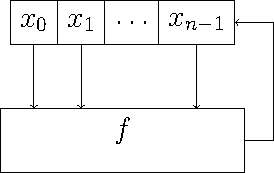
\includegraphics[page=1]{figures/boolean/lfsr.pdf}
	\caption{Feedback Shift Register}
	\label{lfsr:im1}
\end{figure}

Thông qua hàm $f$, các vector trong $\FF_2^n$ sẽ chuyển trạng thái lẫn nhau theo công thức 
\begin{equation}
	(x_{n-1}, x_{n-2}, \ldots, x_1, x_0) \to (x_n, x_{n-1}, \ldots, x_2, x_1)
\end{equation}

\begin{example}
	Xét hàm boolean $f(x_3, x_2, x_1, x_0) = x_3 x_2 \oplus x_0$. Bảng chân trị của hàm $f$ là \[f(x_3, x_2, x_1, x_0) = (0, 1, 0, 1, 0, 1, 0, 1, 0, 1, 0, 1, 1, 0, 1, 0)\]
	
	Ví dụ, với $(0, 0, 0, 1)$, ta có $f(0, 0, 0, 1) = 1$ nên $(0, 0, 0, 1)$ biến đổi thành $(1, 0, 0, 0)$. Như vậy chúng ta có các chuyển đổi đối với hàm $f$ được thể hiện thành 4 chu trình ở hình \ref{lfsr:im2} và \ref{lfsr:im3}.
	
	%\[(0, 0, 0, 0) \to (0, 0, 0, 0)\]
	
	%\[(0, 0, 0, 1) \to (1, 0, 0, 0) \to (0, 1, 0, 0) \to (0, 0, 1, 0) \to (0, 0, 0, 1)\]
	
	%\[(0, 0, 1, 1) \to (1, 0, 0, 1) \to (1, 1, 0, 0) \to (1, 1, 1, 0) \to (1, 1, 1, 1) \to (0, 1, 1, 1) \to (1, 0, 1, 1) \to (1, 1, 0, 1) \to (0, 1, 1, 0) \to (0, 0, 1, 1)\]
	
	%\[(0, 1, 0, 1) \to (1, 0, 1, 0) \to (0, 1, 0, 1)\]
	\begin{figure}[ht]
		\begin{subfigure}{0.4\textwidth}
			\centering
			\includegraphics[page=2]{figures/boolean/lfsr.pdf}
			\caption{Chu trình thứ nhất}
		\end{subfigure}
		\hfill
		\begin{subfigure}{0.4\textwidth}
			\centering
			\includegraphics[page=3]{figures/boolean/lfsr.pdf}
			\caption{Chu trình thứ hai}
		\end{subfigure}
		\caption{Các chu trình chuyển đổi của $f$}
		\label{lfsr:im2}
	\end{figure}
	\begin{figure}[ht]
		\begin{subfigure}{0.3\textwidth}
			\centering
			\includegraphics[page=5]{figures/boolean/lfsr.pdf}
			\caption{Chu trình thứ ba}
		\end{subfigure}
		\hfill
		\begin{subfigure}{0.65\textwidth}
			\centering
			\includegraphics[page=4]{figures/boolean/lfsr.pdf}
			\caption{Chu trình thứ tư}
		\end{subfigure}
		\caption{Các chu trình chuyển đổi của $f$}
		\label{lfsr:im3}
	\end{figure}
	
\end{example}
Ta thấy rằng tập các vector $\bm{x} = (x_i, x_{i+1}, \ldots, x_{i+n-1})$ có $2^n$ trường hợp. Do đó sẽ có một lúc nào đó (số $i$ nào đó) mà vector $\bm{x}$ trở lại đúng vector ban đầu. Nghĩa là tồn tại $i$ sao cho \[(x_0, x_1, \ldots, x_{n-1}) = (x_i, x_{i+1}, \ldots, x_{i+n-1})\] Từ đó dãy bit tiếp theo được sinh ra sẽ giống hệt trước đó nên số $i$ nhỏ nhất thỏa mãn đẳng thức được gọi là \textbf{chu kì} của Feedback Shift Register.

Trong các hàm boolean thì hàm boolean tuyến tính được quan tâm nhiều nhất để sinh ra chuỗi bit Feedback Shift Register. Do đó từ đây ta tập trung vào các hàm boolean tuyến tính và Linear Feedback Shift Register.

Nhắc lại, hàm boolean tuyến tính là hàm boolean có dạng
\begin{equation*}
	f(x_0, x_1, \ldots, x_{n-1}) = a_0 x_0 \oplus a_1 x_1 \oplus \ldots \oplus a_{n-1} x_{n-1}
\end{equation*}
Trong đó $a_i \in \FF_2$ là các hệ số cho trước. Ta định nghĩa đa thức đặc trưng cho hàm boolean tuyến tính như sau.

\begin{definition}[Đa thức đặc trưng]
	Xét hàm boolean tuyến tính \[f(x_0, x_1, \ldots, x_{n-1}) = a_0 x_0 \oplus a_1 x_1 \oplus \ldots \oplus a_{n-1} x_{n-1}\] Khi đó đa thức đặc trưng tương ứng với hàm $f$ là đa thức trong $GF(2^n)$
	\begin{equation}
		P(x) = a_0 + a_1 x + \ldots + a_{n-1} x^{n-1} + x^n
	\end{equation}
\end{definition}

Do hàm boolean tuyến tính có tính chất là $f(\bm{0}) = 0$ nên chu kì tối đa có thể đạt được là $2^n - 1$. Ta có một vài định nghĩa sau để một LFSR đạt được chu kì tối đa.

\begin{definition}[Đa thức primitive]
	Xét đa thức $P(x) = a_0 + a_1 x + \ldots + a_{n-1} x^{n-1} + x^n$ thuộc $GF(2^n)$. Ta đã biết trường $GF(2^n)$ có $2^n - 1$ phần tử khác không. Đặt $p = 2^n - 1$. Đa thức $P(x)$ được gọi là \textbf{primitive} khi với mọi ước nguyên tố $q$ của $p$ thì 
	\begin{equation*}
		x^s \not\equiv 1 \bmod{P(x)}, \quad \text{với } s = \frac{p}{q} = \frac{2^n - 1}{q}
	\end{equation*}
\end{definition}

\begin{definition}[Đa thức đặc trưng với chu kì cực đại]
	Đa thức $P(x) = a_0 + a_1 x + \ldots + a_{n-1} x^{n-1} + x^n$ được gọi là \textbf{đa thức đặc trưng với chu kì cực đại} nếu đa thức đó tối giản và là đa thức primitive. 
\end{definition}

\begin{example}
	Xét đa thức $f(x) = x^4 + x^3 + 1$. Ta có thể xác định xem đa thức này có sinh ra LFSR với chu kì tối đa hay không mà không cần tìm đồ thị chuyển trạng thái của LFSR.
	
	Đầu tiên ta chứng minh $f(x)$ là đa thức tối giản. Thật vậy, giả sử ngược lại, $f(x)$ là tích của hai đa thức bậc nhỏ hơn 4. Hai trường hợp có thể xảy ra là $f(x)$ chia hết cho đa thức tối giản bậc 1 hoặc bậc 2.
	
	Các đa thức tối giản bậc 1 là $x$ và $x+1$. Ta có thể kiểm chứng rằng $f(x)$ không chia hết cho bất kì đa thức nào ở trên. Tương tự, đa thức tối giản bậc 2 (trong $GF(2^4)$) là $x^2 + x + 1$ và $f(x)$ cũng không chia hết cho đa thức này. Như vậy ta có thể kết luận rằng $f(x)$ là đa thức tối giản.
	
	Trong $GF(2^4)$ có $2^4 - 1 = 15$ phần tử khác 0. Các ước nguyên tố của 15 là 3 và 5. Ta thấy rằng $x^3 \not\equiv 1$ và $x^5 = x \cdot x^4 = x \cdot (x^3 + 1) = x^4 + x = x^3 + x + 1 \not\equiv 1$. Như vậy $f(x)$ là đa thức primitive.
	
	Như vậy ta có thể kết luận rằng đa thức $f(x)$ sinh ra LFSR với chu kì tối đa.
\end{example}

